% Artigo do projeto FIEP — compilar com:  latexmk -pdf main.tex   (ou Overleaf: enviar a pasta artigo/)
% Os números, tabelas e figuras de resultados vêm de `fiep experimento --artigo` (pasta gerado/).
\documentclass[11pt,a4paper]{article}

\usepackage[T1]{fontenc}
\usepackage[utf8]{inputenc}
\usepackage[brazilian]{babel}
\usepackage{mathptmx}
\usepackage[a4paper,margin=2.5cm]{geometry}
\usepackage{amsmath}
\usepackage{graphicx}
\usepackage{booktabs}
\usepackage{multirow}
\usepackage{float}
\usepackage[font=small,labelfont=bf]{caption}
\usepackage{subcaption}
\usepackage[numbers,sort&compress]{natbib}
\usepackage{xcolor}
\usepackage{url}
\usepackage[hidelinks]{hyperref}
\usepackage{microtype}

% Trechos que dependem de informação do laboratório aparecem em vermelho.
\newcommand{\preencher}[1]{\textcolor{red}{[\textbf{preencher:} #1]}}

% Números do experimento (gerado por fiep experimento --artigo)
\IfFileExists{gerado/tabelas/numeros.tex}{% Gerado automaticamente por fiep experimento — não edite à mão
\newcommand{\ExpId}{20261020-121224}
\newcommand{\TipoTeste}{20\% das amostras separadas antes do treino (estratificado)}
\newcommand{\NAmostrasTreino}{160}
\newcommand{\NAmostrasTeste}{40}
\newcommand{\NReplicasTreino}{402}
\newcommand{\NReplicasTeste}{100}
\newcommand{\NCombinacoes}{60}
\newcommand{\MelhorModelo}{log\_reg\_l1}
\newcommand{\MelhorVariante}{dif\_curva\_linha\_base}
\newcommand{\ABcv}{0,948}
\newcommand{\ABcvDP}{0,022}
\newcommand{\AUCcv}{0,977}
\newcommand{\ABteste}{0,946}
\newcommand{\SENSteste}{0,934}
\newcommand{\ESPECteste}{0,958}
\newcommand{\AUCteste}{0,983}
\newcommand{\Limiar}{0,68}
\newcommand{\RegModelo}{ridge}
\newcommand{\RegRMSEcv}{0,79}
\newcommand{\RegRMSEteste}{0,81}
\newcommand{\RegRdoisTeste}{0,66}
\newcommand{\FormulaSISSO}{\texttt{\small p(contaminada) = $\sigma$(-0.887$\cdot$[(rRNA i\_pico-sonda i\_pico)] -0.719$\cdot$[($\Delta$area\_rRNA vs carbono-$\Delta$e\_pico\_rRNA vs sonda)] +0.353)}}
}{%
  \newcommand{\ABteste}{--}\newcommand{\ABcv}{--}\newcommand{\MelhorModelo}{--}}
\graphicspath{{gerado/figuras/}}

\title{Detecção de contaminação microbiana em superfícies por biossensores
eletroquímicos impressos e aprendizado de máquina}
\author{\preencher{autores e afiliações}\\
\small Instituto SENAI de Inovação \preencher{unidade} \quad
\small Projeto FIEP}
\date{}

\begin{document}
\maketitle

\begin{abstract}
O monitoramento microbiológico de superfícies na indústria depende hoje de plaqueamento, que leva
dias para gerar resultado. Este trabalho apresenta uma plataforma que combina biossensores
eletroquímicos impressos (eletrodos de carbono com sonda de captura para rRNA 16S), aquisição por
voltametria de pulso diferencial (DPV) e aprendizado de máquina para classificar superfícies como
contaminadas ou não contaminadas e estimar a carga bacteriana. Os voltamogramas são lidos
diretamente dos arquivos do potenciostato, passam por controle de qualidade automático e são
organizados em um banco de dados rastreável. A característica mais informativa foi a curva de
diferença entre estágios do sensor no mesmo eletrodo (antes e depois do contato com o alvo).
Foram comparadas \NCombinacoes{} combinações de pré-processamento e modelo por validação cruzada
agrupada por amostra; o modelo escolhido (\MelhorModelo, \MelhorVariante) obteve acurácia
balanceada de \ABcv{} na validação cruzada e de \ABteste{} no conjunto de teste
(\TipoTeste), com AUC de \AUCteste. A carga bacteriana das amostras contaminadas foi estimada com
RMSE de \RegRMSEteste{} log$_{10}$\,UFC/mL. \preencher{revisar após o experimento com os dados
reais das empresas validadoras}

\medskip\noindent\textbf{Palavras-chave:} biossensor eletroquímico; voltametria de pulso
diferencial; rRNA 16S; aprendizado de máquina; monitoramento de superfícies; ISO 18593.
\end{abstract}

\section{Introdução}

A verificação da higiene de superfícies em linhas de produção é exigida em programas de segurança
de alimentos e de controle de contaminação. Os métodos de referência, baseados na coleta de
amostras de superfície \citep{iso18593} e no cultivo em placa, são confiáveis, mas o resultado
demora de um a vários dias, o que impede uma decisão no mesmo turno de produção.

Biossensores eletroquímicos de DNA (genossensores) detectam sequências específicas de
microrganismos, como trechos do gene do rRNA 16S, por meio de uma sonda de captura imobilizada no
eletrodo: a hibridização com o alvo altera a transferência de carga de uma sonda redox em solução
(por exemplo, o par ferri/ferrocianeto), o que aparece como mudança na corrente de pico do
voltamograma. Eletrodos impressos de carbono (SPCE) tornam a medição barata e portátil, mas o
sinal varia entre eletrodos, lotes e operadores, e a decisão por um limiar fixo de corrente tende a
falhar fora do laboratório.

Técnicas de aprendizado de máquina e quimiometria têm sido usadas para extrair mais informação de
sinais eletroquímicos, de PCA e PLS a florestas aleatórias, máquinas de vetores de suporte e redes
neurais \citep{puthongkham2021, bocan2025}. Duas dificuldades se repetem nesses trabalhos: os
conjuntos de dados são pequenos e heterogêneos, e a validação nem sempre impede que medições da
mesma amostra apareçam no treino e no teste, o que infla os resultados \citep{kapoor2023}. Métodos
que produzem descritores explícitos, como o SISSO \citep{ouyang2018}, são atraentes nesse cenário
porque funcionam com poucas amostras e dão uma fórmula interpretável.

Este trabalho descreve uma plataforma integrada, desenvolvida no projeto FIEP, com os seguintes
objetivos: (i) ler os voltamogramas diretamente dos arquivos do potenciostato e organizá-los em um
banco de dados rastreável, com controle de qualidade automático; (ii) comparar de forma sistemática
representações do sinal e modelos supervisionados, incluindo o SISSO, para classificar superfícies
e estimar a carga bacteriana; e (iii) disponibilizar o modelo escolhido em uma ferramenta de uso no
laboratório e nas empresas validadoras.

\section{Materiais e métodos}

\subsection{Biossensor e aquisição}
Os sensores são eletrodos impressos de carbono fabricados por serigrafia em escala piloto
\preencher{fabricante/processo, área do eletrodo de trabalho, referência e contraeletrodo}. Cada
eletrodo é medido em três etapas sucessivas da montagem do sensor, e a informação usada pelo modelo
é a mudança entre a última etapa (após o contato com a amostra) e a anterior, no mesmo eletrodo.
Dois protocolos estão previstos na pipeline: o biossensor genossensor para rRNA 16S, com carbono
limpo, sonda de captura e sonda após a incubação com a amostra, medido por voltametria de pulso
diferencial (DPV); e o imunossensor para NS1, com bloqueio, imobilização do anticorpo monoclonal
(mAb-NS1) e etapa final, medido por voltametria de onda quadrada (SWV). \preencher{protocolo
usado nos resultados, sequência e concentração da sonda ou do anticorpo}
As medições foram feitas em \preencher{eletrólito} com
ferri/ferrocianeto \preencher{concentração} em um potenciostato Metrohm Autolab controlado pelo
software NOVA 2, com faixa de potencial de \preencher{início} a \preencher{fim} V, passo de
\preencher{passo} V, amplitude de modulação de \preencher{amplitude} V e tempo de modulação de
\preencher{tempo} s.

\subsection{Amostragem e referência microbiológica}
As superfícies foram amostradas segundo a ISO~18593 \citep{iso18593} \preencher{método: swab ou
esponja, área amostrada, número de pontos, empresas e tipos de superfície}. A carga bacteriana de
referência foi obtida por plaqueamento em triplicata \preencher{meio, diluições, incubação}, e a
amostra foi rotulada como contaminada quando \preencher{critério}. A carga em
log$_{10}$\,UFC/mL foi usada como alvo da regressão.

\subsection{Leitura dos arquivos e banco de dados}
Os arquivos \texttt{.nox} gerados pelo NOVA são serializações binárias do .NET; a pipeline os lê
diretamente, sem depender do software do fabricante, implementando o formato MS-NRBF
\citep{msnrbf}. De cada medição são extraídos o potencial aplicado, a corrente diferencial
($\delta i$) e, para o controle de qualidade, o potencial efetivamente medido no eletrodo e a
corrente de base; exportações do NOVA em Excel ou CSV também são aceitas. A amostra, o eletrodo e a
etapa do sensor são deduzidos da organização das pastas, do nome do arquivo e do cabeçalho do
\texttt{.nox}, com conferência por planilha. Os dados são gravados em um banco relacional (modelo
ORM com migrações versionadas) com tabelas de empresas, coletas, amostras, plaqueamentos,
medições, curvas, controle de qualidade, modelos e previsões; cada arquivo importado é registrado
pelo seu hash SHA-256, o que garante rastreabilidade e evita duplicidade. Os colaboradores enviam
as coletas por uma plataforma web com autenticação, que grava no mesmo banco.

\subsection{Controle de qualidade}
Cada medição é reprovada automaticamente quando: tem menos de 50 pontos ou mais de 2\% de pontos
inválidos; a corrente bruta ultrapassa 5~mA (sobrecarga do canal de corrente); ou o potencial
medido se afasta do aplicado em mais de 20~mV em mais de 5\% dos pontos, descontado o
deslocamento constante da amplitude do pulso na SWV (o potenciostato não manteve o potencial). Medições com corrente máxima acima de dez vezes a mediana das medições da mesma técnica
e estágio são marcadas para revisão. O resultado é combinado com a marcação manual do laboratório,
prevalecendo a mais restritiva. Só medições aprovadas entram no treino e na previsão.

\subsection{Pré-processamento e características}
Cada voltamograma é interpolado em uma grade comum de potencial (definida no treino e reutilizada
na previsão) e suavizado por Savitzky--Golay \citep{savitzky1964} (janela 11, ordem 3).
Opcionalmente, remove-se uma linha de base linear ajustada aos 10\% de pontos de cada extremo.
Foram comparadas cinco representações (Tabela~\ref{tab:variantes}). A hipótese central é que a
\emph{diferença} entre o último e o penúltimo estágio do mesmo eletrodo isola o efeito da
hibridização e cancela a variação entre eletrodos.

\begin{table}[H]
\centering\small
\caption{Representações do sinal comparadas.}\label{tab:variantes}
\begin{tabular}{lp{10cm}}
\toprule
Variante & Descrição \\ \midrule
\texttt{dif\_resumo} & descritores de cada estágio (corrente e potencial de pico, área, largura a
meia altura) e suas diferenças entre estágios \\
\texttt{dif\_curva} & idem, mais a curva de diferença completa (último $-$ penúltimo estágio) \\
\texttt{dif\_curva\_linha\_base} & \texttt{dif\_curva} com remoção de linha de base linear \\
\texttt{dif\_curva\_sem\_suavizar} & \texttt{dif\_curva} sem suavização \\
\texttt{estagio\_final} & apenas o estágio final, sem informação dos estágios anteriores \\
\bottomrule
\end{tabular}
\end{table}

\subsection{Modelos e protocolo de validação}
Foram avaliados regressão logística (regularização L2 com três intensidades e L1), análise
discriminante linear com encolhimento, SVM com núcleo RBF (calibrada), $k$ vizinhos mais
próximos, floresta aleatória \citep{breiman2001}, \textit{extra trees}, \textit{gradient boosting}
baseado em histogramas e uma versão simplificada do SISSO \citep{ouyang2018}, todos implementados
com o scikit-learn \citep{pedregosa2011}. No SISSO simplificado, os descritores primários
padronizados geram um espaço de candidatos por uma aplicação dos operadores
$\{x, x^2, \sqrt{|x|}, \log|x|, x_i - x_j, x_i x_j, x_i/x_j\}$; a triagem por independência
segura \citep{fan2008} mantém os 25 candidatos de maior separação entre as classes (AUC) e uma
busca exaustiva escolhe a combinação de até dois candidatos com maior acurácia balanceada em uma
regressão logística.

Antes de qualquer ajuste, as amostras são divididas em três conjuntos --- treino
(\PropTreino\%), validação (\PropValidacao\%) e teste (\PropTeste\%) ---, a divisão típica
sugerida por \citet[seção~7.2]{hastie2009}: o treino ajusta os modelos, a validação escolhe entre
eles e o teste estima o erro de generalização do modelo escolhido. A divisão é feita por amostra
(todas as réplicas e estágios de uma amostra ficam no mesmo conjunto), estratificada pela classe,
para que medições da mesma amostra não apareçam em conjuntos diferentes \citep{kapoor2023}. Coletas
reservadas para validação externa (por exemplo, de outra empresa) entram inteiras no teste.

No treino, cada combinação de representação e modelo é avaliada também por validação cruzada em
cinco dobras agrupadas por amostra (\textit{StratifiedGroupKFold}), que dá a estabilidade do
desempenho e o limiar de decisão --- o que maximiza o índice J de Youden \citep{youden1950} nas
previsões fora da dobra. O modelo ajustado no treino classifica a validação com esse limiar, e a
combinação escolhida é a de maior acurácia balanceada na validação (\CriterioEscolha). Só então a
combinação é re-treinada com treino e validação juntos e avaliada uma única vez no teste, que não
participa de nenhuma escolha \citep{raschka2018,vabalas2019}. Para a regressão da carga, usam-se as
amostras contaminadas, o mesmo protocolo (escolha pelo RMSE na validação) e os modelos Ridge, PLS,
SVR, floresta aleatória, \textit{extra trees} e \textit{gradient boosting}.

Como cada amostra é medida em vários eletrodos, a decisão final por amostra usa a média das
probabilidades das réplicas aprovadas no controle de qualidade. Nas amostras classificadas como
contaminadas, a carga estimada pode ser convertida em níveis de contaminação por limites de
log$_{10}$\,UFC/mL definidos pela equipe. \preencher{limites dos níveis (baixa, moderada, alta), se
adotados}

As métricas de classificação são a acurácia balanceada (AB, média de sensibilidade e
especificidade, adequada a classes desbalanceadas), sensibilidade, especificidade e área sob a
curva ROC (AUC); para a regressão, RMSE, MAE e $R^2$ em log$_{10}$\,UFC/mL.

\section{Resultados}

\noindent\preencher{Os números abaixo são gerados automaticamente pelo último
\texttt{fiep experimento --artigo} (experimento \ExpId). Enquanto os dados das empresas não forem
incorporados, eles se referem ao conjunto de demonstração do projeto; apagar esta nota ao usar os
dados reais.}

\subsection{Conjunto de dados e controle de qualidade}
O conjunto de treino teve \NAmostrasTreino{} amostras (\NReplicasTreino{} réplicas com os três
estágios aprovados no controle de qualidade) e o de teste \NAmostrasTeste{} amostras
(\NReplicasTeste{} réplicas), separado como \TipoTeste. \preencher{número de medições reprovadas
no controle de qualidade e principais motivos, a partir de \texttt{fiep db resumo}}

\subsection{Efeito da hibridização no sinal}
A Figura~\ref{fig:curvas} mostra a curva média de diferença entre o último e o penúltimo estágio.
Nas amostras contaminadas, a corrente diminui na região do pico do par ferri/ferrocianeto, o que é
compatível com o bloqueio da transferência de carga após a hibridização do alvo.

\begin{figure}[H]
\centering
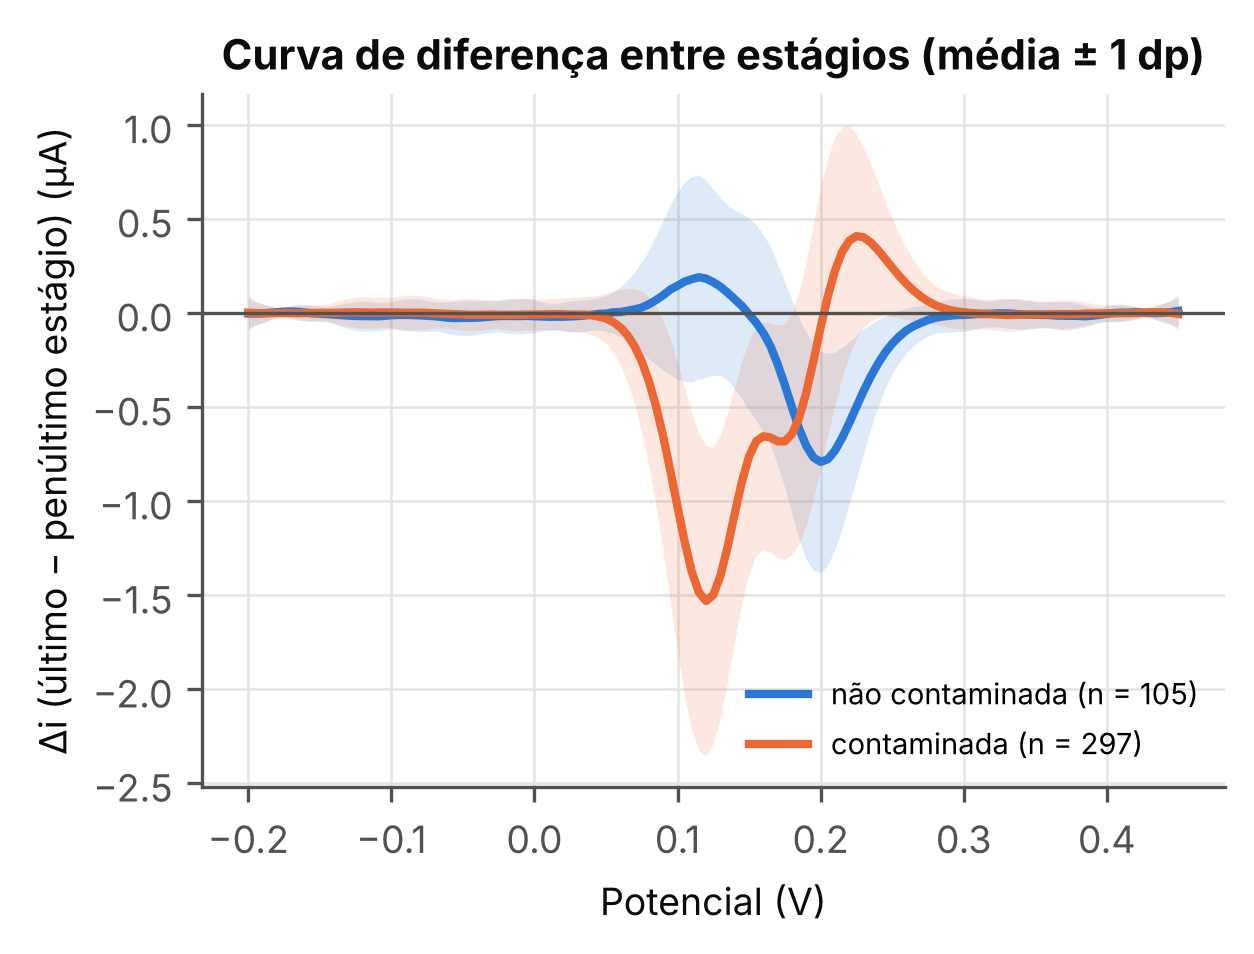
\includegraphics[width=0.62\textwidth]{curvas_diferenca.png}
\caption{Curva de diferença entre estágios (média $\pm$ 1 desvio-padrão) por classe, conjunto de treino.}
\label{fig:curvas}
\end{figure}

\subsection{Comparação de representações e modelos}
Foram avaliadas \NCombinacoes{} combinações (Figura~\ref{fig:comparacao},
Tabela~\ref{tab:classificacao}). A combinação escolhida pela validação cruzada foi
\MelhorModelo{} com a representação \MelhorVariante, com acurácia balanceada de
\ABcv{} $\pm$ \ABcvDP{} e AUC de \AUCcv. No conjunto de teste, ela obteve acurácia balanceada de
\ABteste, sensibilidade de \SENSteste, especificidade de \ESPECteste{} e AUC de \AUCteste{}
(limiar de \Limiar).

\begin{figure}[H]
\centering
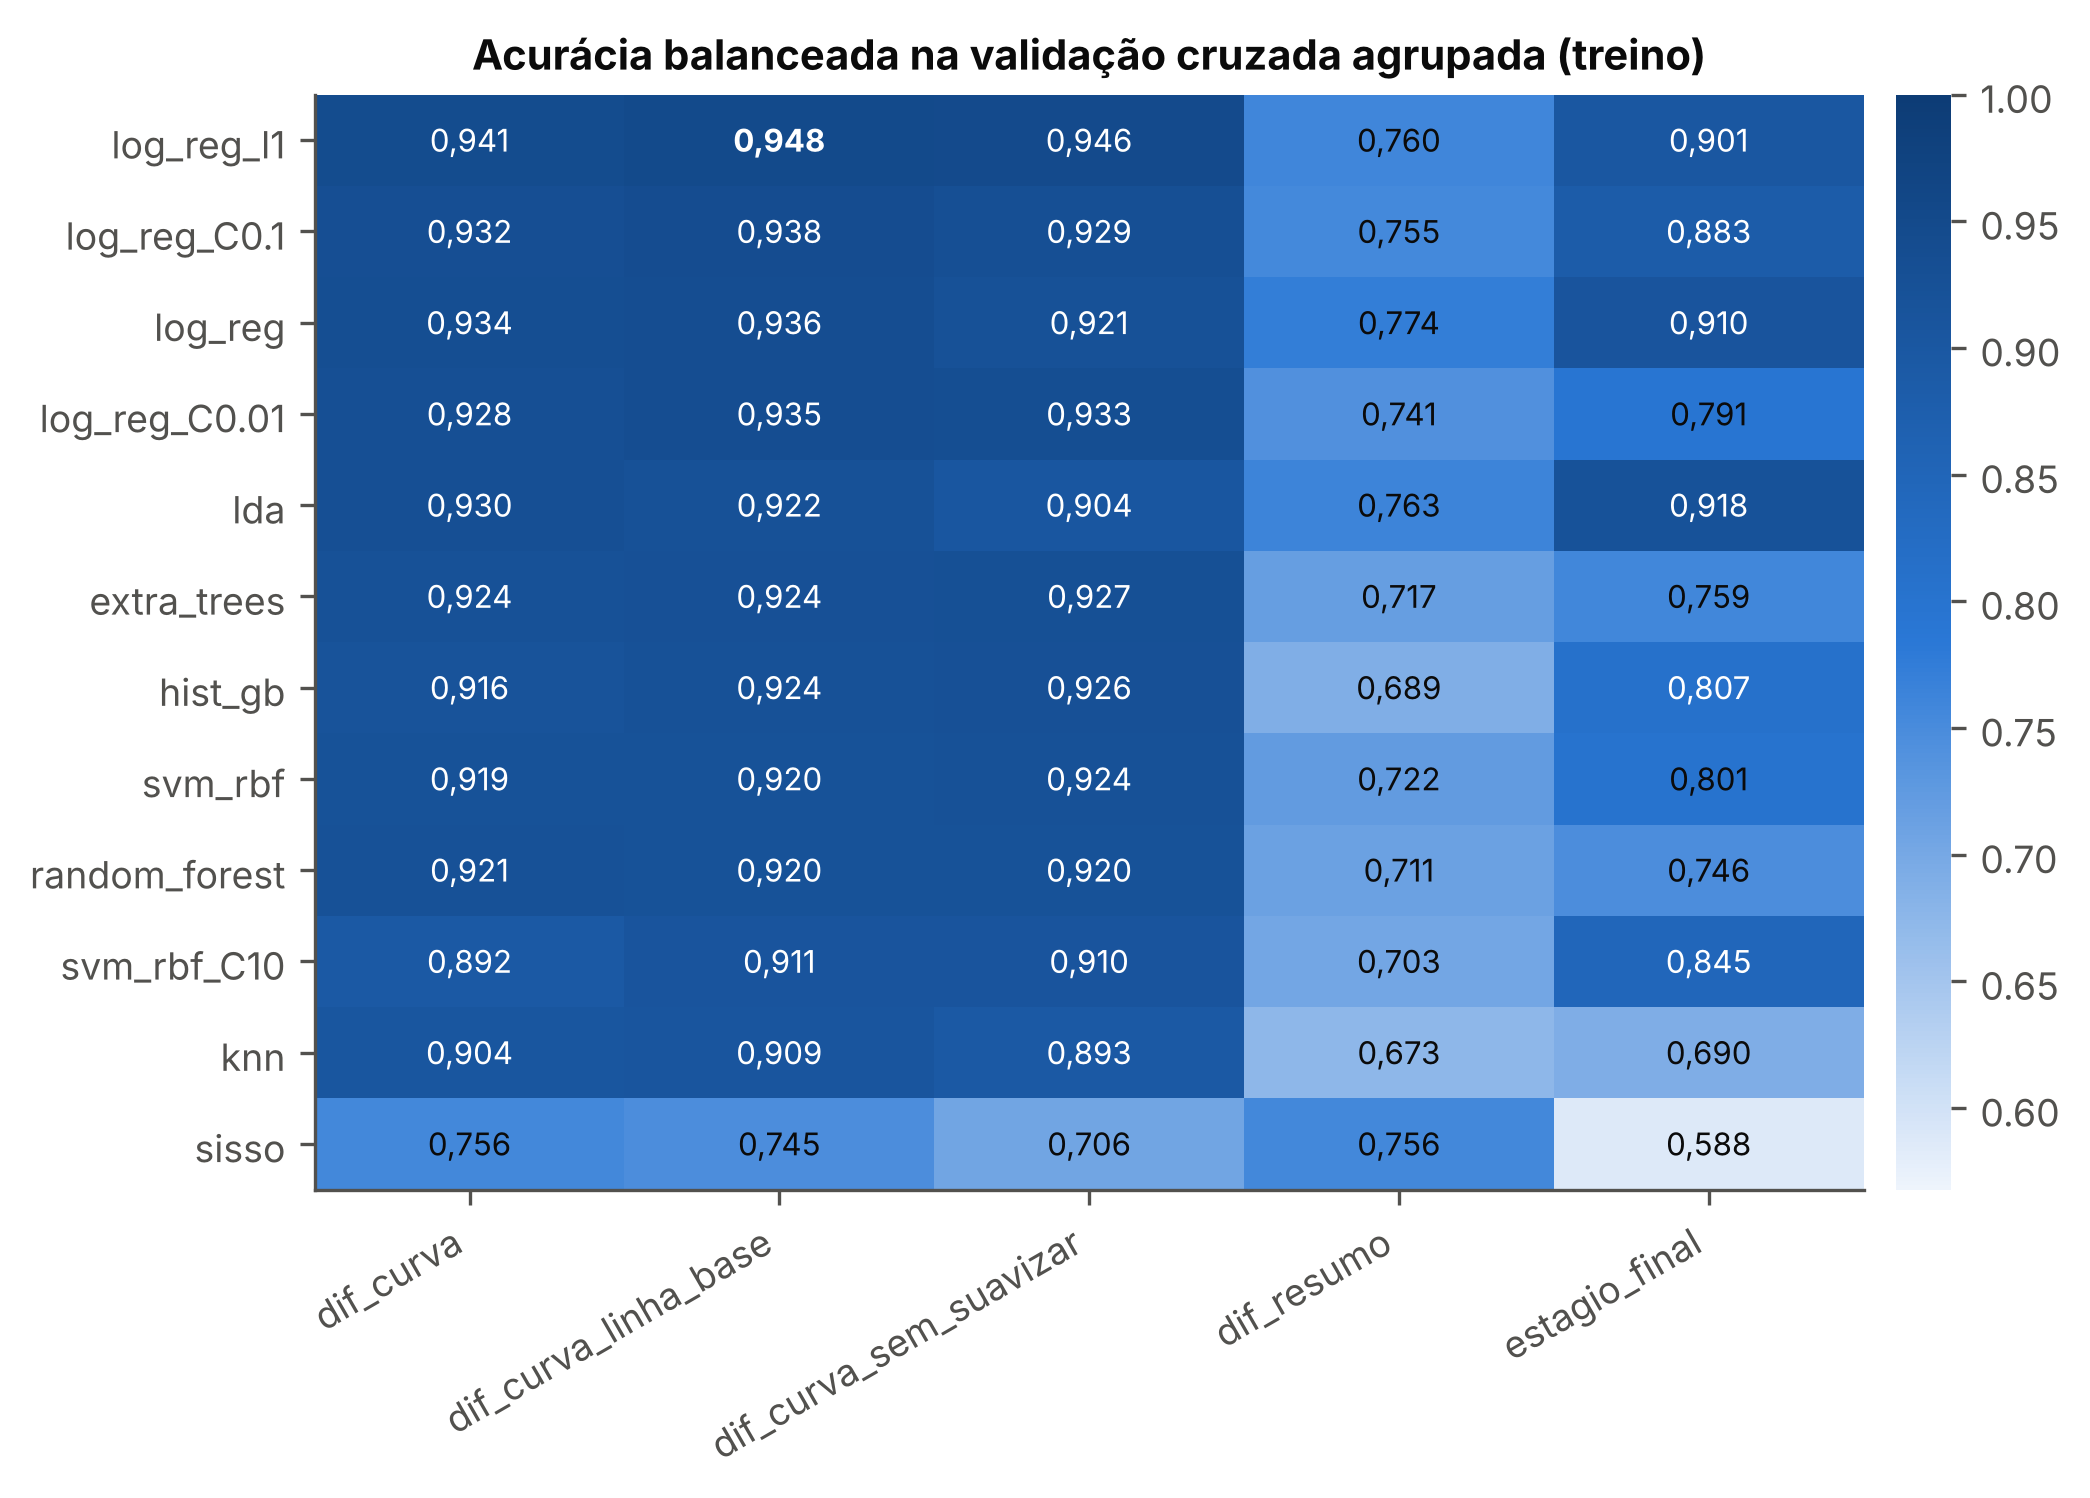
\includegraphics[width=0.9\textwidth]{comparacao_modelos.png}
\caption{Acurácia balanceada média na validação cruzada agrupada (treino) para cada representação e modelo.}
\label{fig:comparacao}
\end{figure}

\begin{table}[H]
\centering\footnotesize
\caption{Dez melhores combinações pela validação cruzada no treino e o desempenho de cada uma no
teste. AB: acurácia balanceada (média $\pm$ desvio-padrão entre dobras).}
\label{tab:classificacao}
\IfFileExists{gerado/tabelas/tabela_classificacao.tex}{\begin{tabular}{rllccccccc}
\toprule
 & & & CV (treino) & \multicolumn{2}{c}{Validação} & \multicolumn{4}{c}{Teste} \\
\cmidrule(lr){4-4}\cmidrule(lr){5-6}\cmidrule(lr){7-10}
\# & Variante & Modelo & AB & AB & AUC & AB & Sens. & Espec. & AUC \\
\midrule
1 & dif\_curva\_sem\_suavizar & log\_reg\_l1 & 0,941 $\pm$ 0,014 & 0,962 & 0,973 & 0,916 & 0,860 & 0,971 & 0,959 \\
2 & dif\_curva\_sem\_suavizar & log\_reg & 0,957 $\pm$ 0,019 & 0,957 & 0,971 & 0,889 & 0,892 & 0,886 & 0,941 \\
3 & dif\_curva\_sem\_suavizar & log\_reg\_C0.1 & 0,941 $\pm$ 0,017 & 0,952 & 0,973 & 0,921 & 0,871 & 0,971 & 0,951 \\
4 & dif\_curva\_linha\_base & log\_reg\_C0.01 & 0,938 $\pm$ 0,025 & 0,952 & 0,970 & 0,937 & 0,903 & 0,971 & 0,954 \\
5 & dif\_curva & lda & 0,955 $\pm$ 0,037 & 0,941 & 0,976 & 0,935 & 0,871 & 1,000 & 0,971 \\
6 & dif\_curva & log\_reg\_C0.1 & 0,941 $\pm$ 0,030 & 0,931 & 0,973 & 0,918 & 0,892 & 0,943 & 0,959 \\
7 & dif\_curva\_linha\_base & lda & 0,952 $\pm$ 0,037 & 0,930 & 0,974 & 0,930 & 0,860 & 1,000 & 0,970 \\
8 & dif\_curva & log\_reg\_l1 & 0,938 $\pm$ 0,019 & 0,926 & 0,973 & 0,903 & 0,892 & 0,914 & 0,960 \\
9 & dif\_curva & log\_reg & 0,949 $\pm$ 0,041 & 0,926 & 0,973 & 0,875 & 0,892 & 0,857 & 0,955 \\
10 & dif\_curva\_linha\_base & log\_reg\_l1 & 0,949 $\pm$ 0,033 & 0,925 & 0,974 & 0,918 & 0,892 & 0,943 & 0,958 \\
\bottomrule
\end{tabular}
}{\preencher{rodar fiep experimento --artigo}}
\end{table}

\begin{figure}[H]
\centering
\begin{subfigure}{0.48\textwidth}\centering
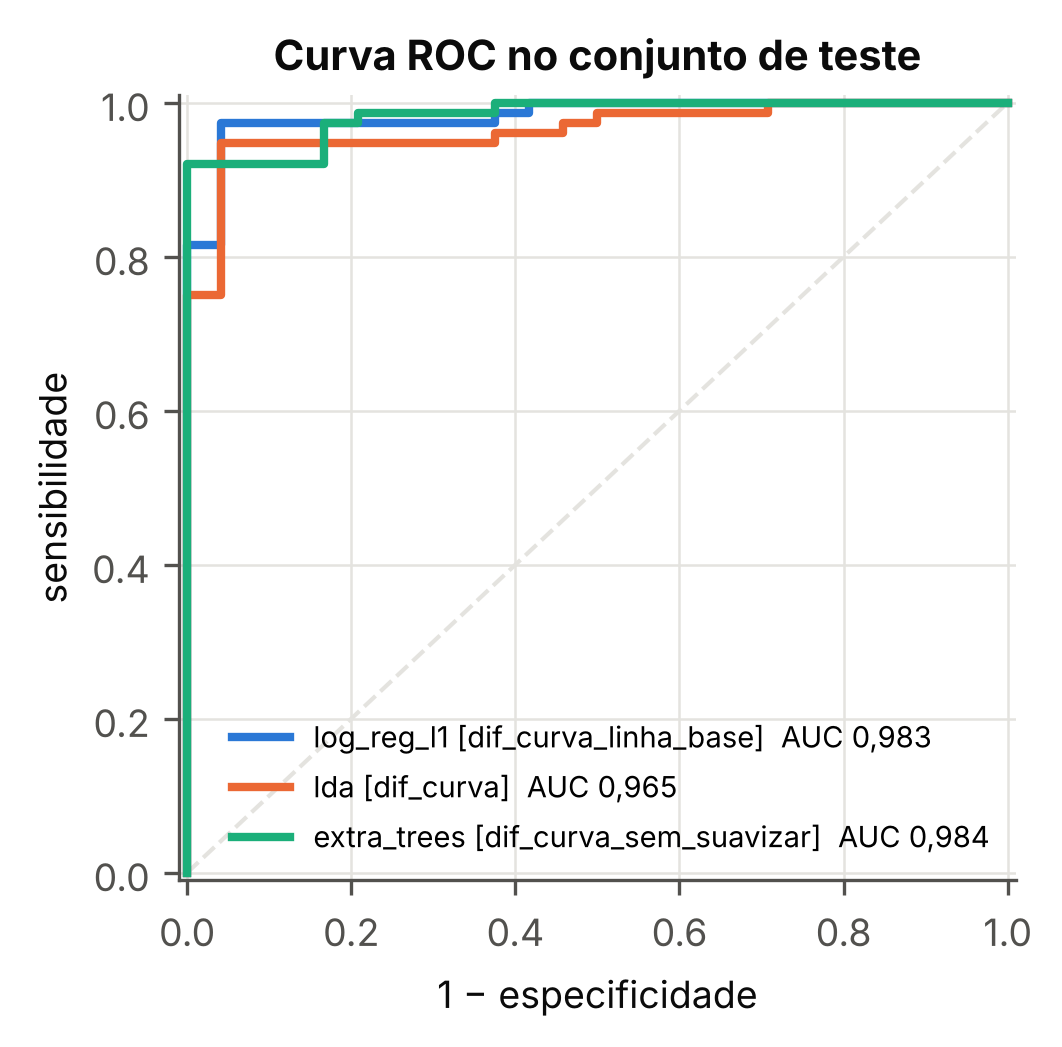
\includegraphics[width=\textwidth]{roc_teste.png}\caption{Curvas ROC no teste.}\end{subfigure}
\hfill
\begin{subfigure}{0.42\textwidth}\centering
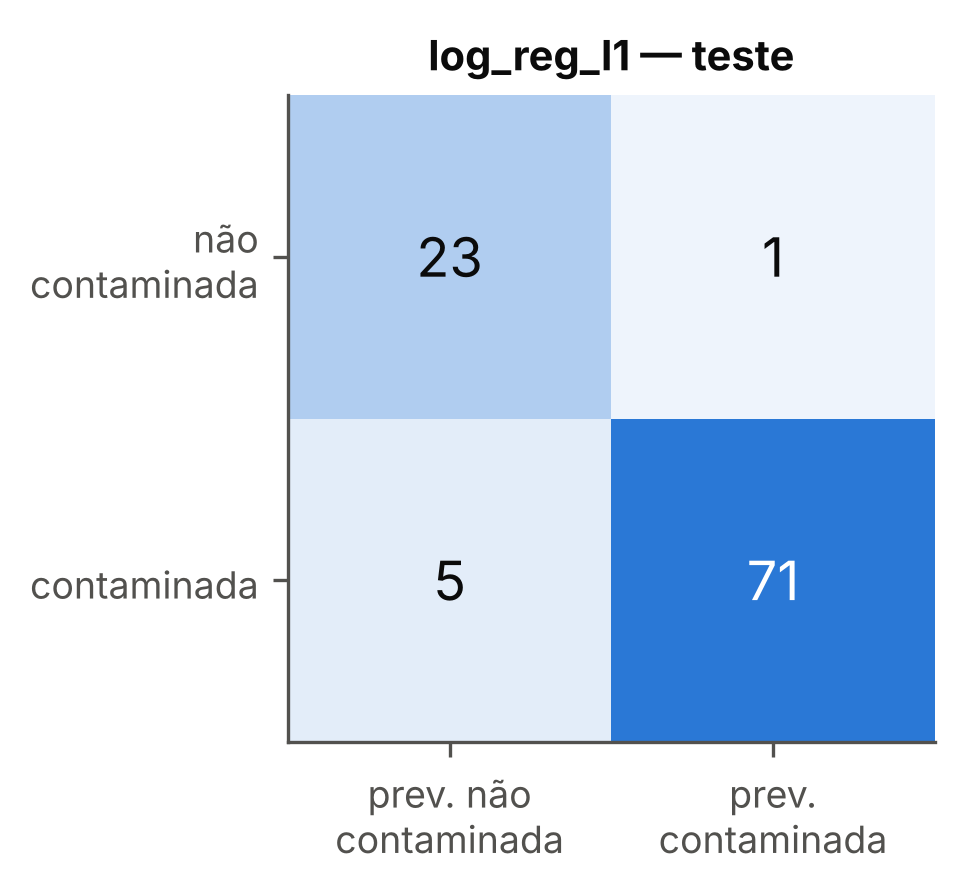
\includegraphics[width=\textwidth]{matriz_confusao_teste.png}\caption{Matriz de confusão do modelo escolhido.}\end{subfigure}
\caption{Desempenho no conjunto de teste.}
\label{fig:teste}
\end{figure}

\subsection{Interpretação}
A importância por permutação (Figura~\ref{fig:importancia}) indica as regiões de potencial que mais
pesam na decisão. O SISSO simplificado encontrou o descritor
\begin{center}\small\FormulaSISSO\end{center}
cuja forma explícita permite discutir o mecanismo com a equipe experimental.

\begin{figure}[H]
\centering
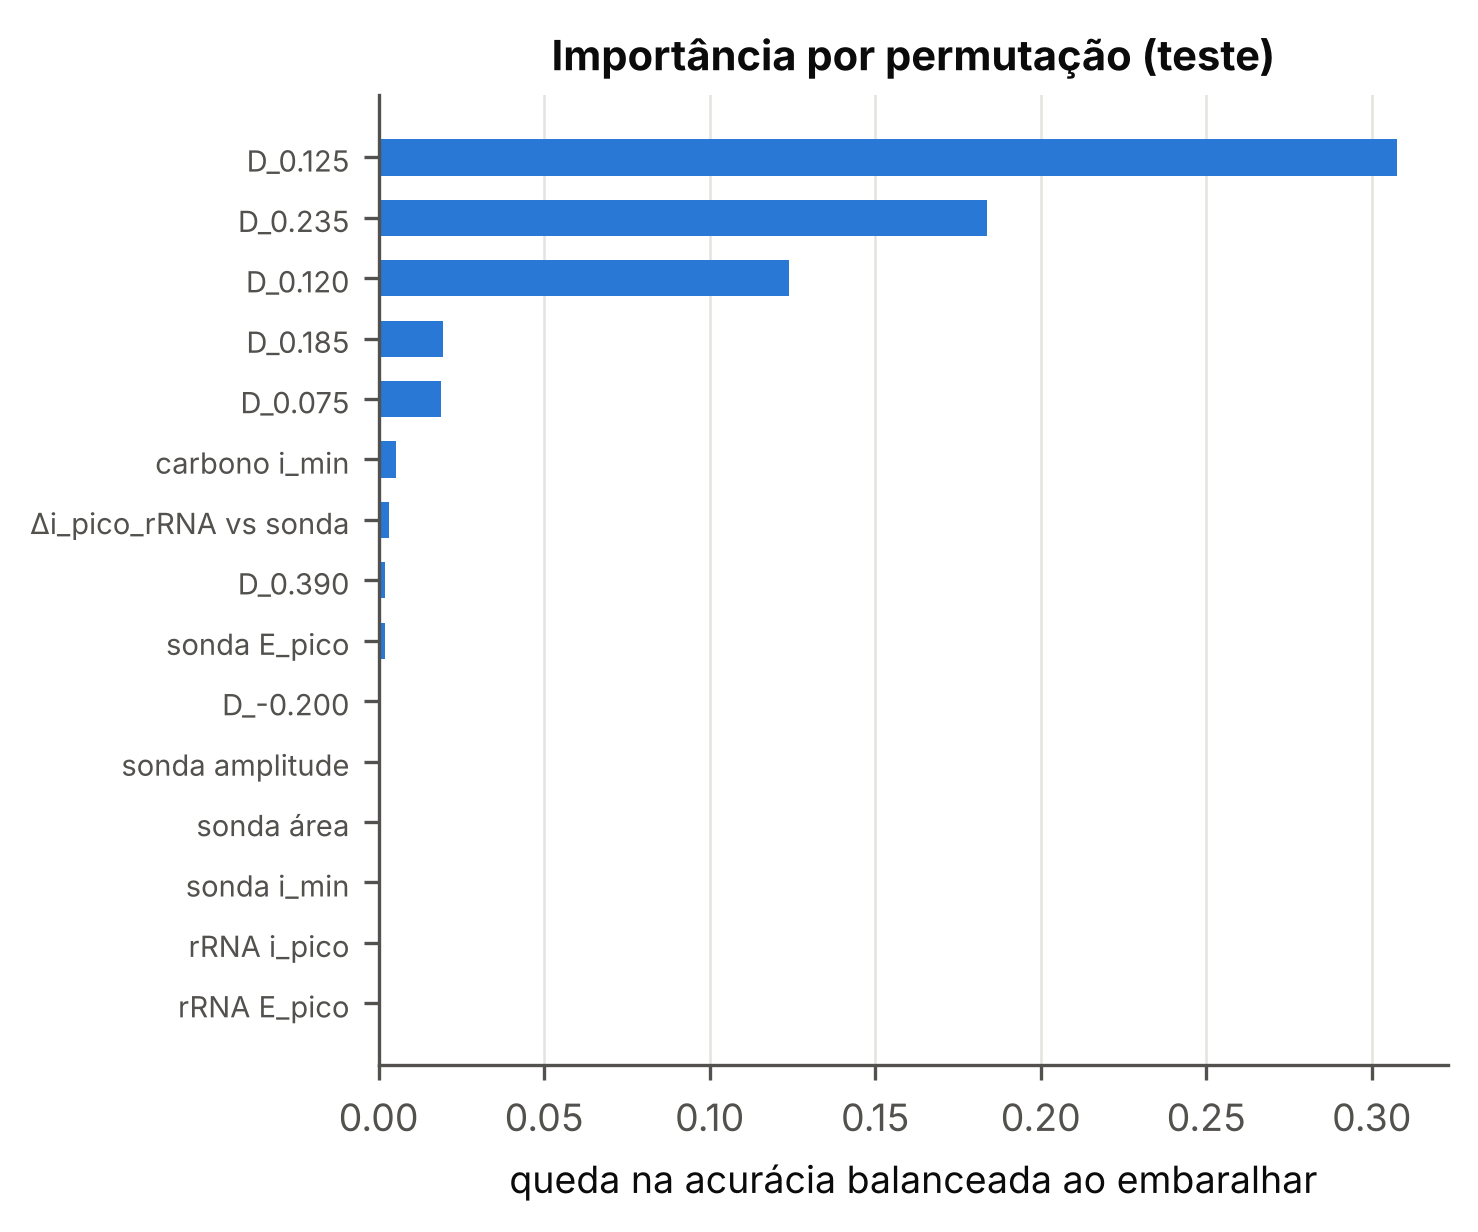
\includegraphics[width=0.6\textwidth]{importancia.png}
\caption{Importância por permutação das características no conjunto de teste (queda da acurácia balanceada).}
\label{fig:importancia}
\end{figure}

\subsection{Estimativa da carga bacteriana}
Nas amostras contaminadas, o melhor regressor (\RegModelo) teve RMSE de \RegRMSEcv{}
log$_{10}$\,UFC/mL na validação cruzada e de \RegRMSEteste{} no teste ($R^2 = \RegRdoisTeste$)
(Tabela~\ref{tab:regressao}, Figura~\ref{fig:regressao}).

\begin{table}[H]
\centering\small
\caption{Regressão da carga bacteriana (log$_{10}$\,UFC/mL) nas amostras contaminadas.}
\label{tab:regressao}
\IfFileExists{gerado/tabelas/tabela_regressao.tex}{\begin{tabular}{llcccc}
\toprule
 & & \multicolumn{2}{c}{Validação cruzada} & \multicolumn{2}{c}{Teste} \\
\cmidrule(lr){3-4}\cmidrule(lr){5-6}
Variante & Modelo & RMSE & $R^2$ & RMSE & $R^2$ \\
\midrule
dif\_curva\_linha\_base & ridge & 0,79 & 0,72 & 0,81 & 0,66 \\
dif\_curva\_linha\_base & pls & 0,82 & 0,70 & 0,86 & 0,61 \\
dif\_curva\_linha\_base & svr & 0,92 & 0,62 & 0,92 & 0,55 \\
dif\_curva\_linha\_base & hist\_gb & 0,93 & 0,62 & 1,05 & 0,42 \\
dif\_curva\_linha\_base & extra\_trees & 0,98 & 0,58 & 1,05 & 0,42 \\
dif\_curva\_linha\_base & random\_forest & 1,01 & 0,55 & 1,10 & 0,36 \\
dif\_resumo & ridge & 1,06 & 0,50 & 1,02 & 0,45 \\
dif\_resumo & pls & 1,06 & 0,50 & 1,05 & 0,42 \\
dif\_resumo & extra\_trees & 1,13 & 0,44 & 1,20 & 0,24 \\
dif\_resumo & random\_forest & 1,15 & 0,41 & 1,30 & 0,11 \\
dif\_resumo & hist\_gb & 1,16 & 0,41 & 1,20 & 0,24 \\
dif\_resumo & svr & 1,27 & 0,29 & 1,39 & -0,02 \\
\bottomrule
\end{tabular}
}{\preencher{rodar fiep experimento --artigo}}
\end{table}

\begin{figure}[H]
\centering
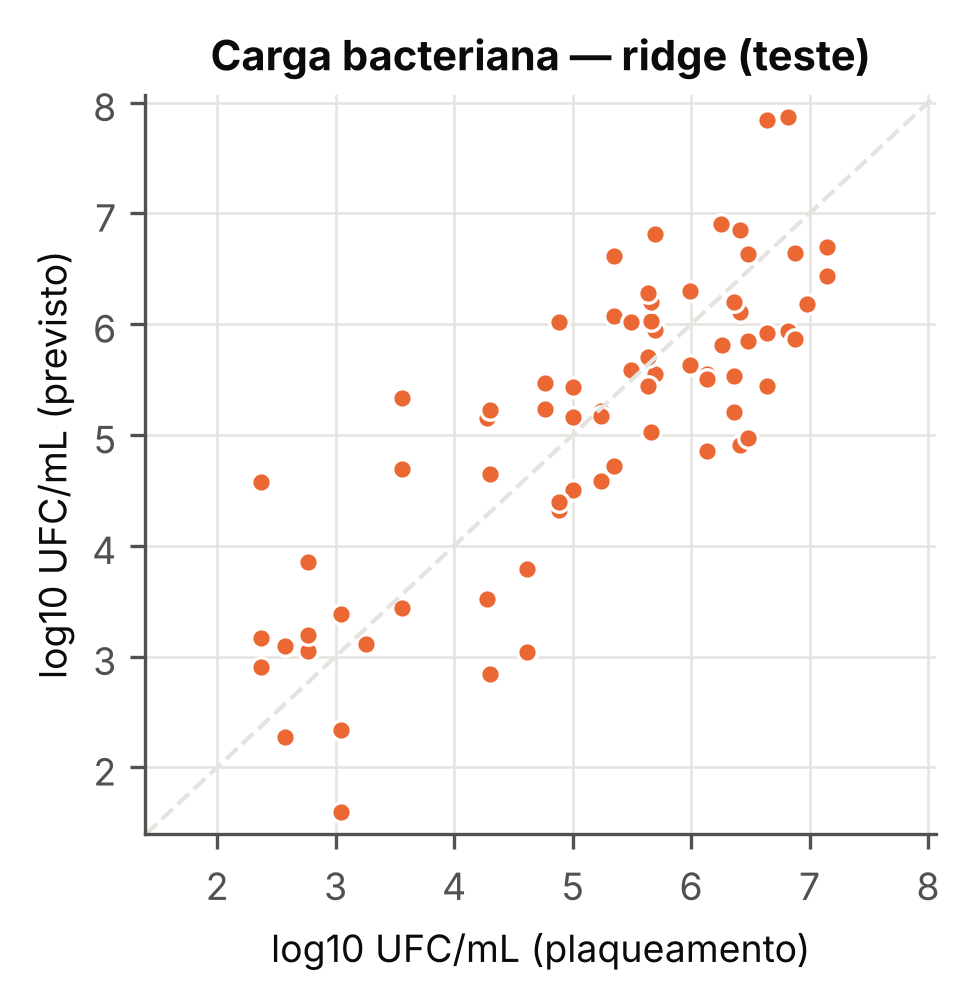
\includegraphics[width=0.45\textwidth]{regressao_teste.png}
\caption{Carga prevista versus plaqueamento no conjunto de teste.}
\label{fig:regressao}
\end{figure}

\section{Discussão}

A diferença entre estágios no mesmo eletrodo foi a representação mais informativa: usar apenas o
estágio final, ou só descritores resumidos do pico, reduziu o desempenho. Isso é coerente com o
princípio do sensor, em que o sinal de interesse é a mudança provocada pela hibridização, e não o
valor absoluto da corrente, que varia entre eletrodos e lotes. Na prática, o protocolo de
aquisição precisa garantir que os três estágios sejam medidos no mesmo eletrodo e registrados na
planilha de metadados; réplicas incompletas não podem ser classificadas.

O controle de qualidade automático se mostrou necessário já nos primeiros arquivos reais do
projeto, em que medições com sobrecarga do canal de corrente e com o potencial medido muito
diferente do aplicado produziam curvas sem significado eletroquímico. Sem esse filtro, essas
medições entrariam no treino como se fossem amostras. \preencher{quantificar com os dados reais}

A validação agrupada por amostra e a separação do teste antes de qualquer escolha evitam o
vazamento de informação entre treino e teste, problema frequente em aplicações de aprendizado de
máquina \citep{kapoor2023}. Como dezenas de combinações foram comparadas, a acurácia da melhor
combinação na validação cruzada tende a ser otimista; o valor de referência é o do conjunto de teste.

\paragraph{Limitações.} \preencher{número de empresas, tipos de superfície e bactérias; variação
entre lotes de eletrodos; necessidade de validação em campo (objetivo 7 do projeto); comparação com
métodos rápidos comerciais, se houver}

\section{Conclusão}

Foi desenvolvida uma plataforma que vai do arquivo do potenciostato à decisão sobre a superfície:
leitura direta dos arquivos do NOVA, controle de qualidade automático, banco de dados rastreável,
comparação sistemática de representações e modelos com validação agrupada e uma ferramenta web para
uso no laboratório e nas empresas validadoras. A curva de diferença entre estágios do sensor,
combinada com \MelhorModelo, classificou as superfícies com acurácia balanceada de \ABteste{} no
conjunto de teste. \preencher{próximos passos: validação em campo nas empresas, ampliação do banco,
estudo da estabilidade entre lotes de eletrodos}


\section*{Disponibilidade de código e dados}
O código da pipeline (leitura dos arquivos do potenciostato, controle de qualidade, banco de dados,
experimentos, API) está disponível em
\url{https://github.com/brunoribas68/bolsa_fiep_-RP_20061}. \preencher{política de disponibilidade dos dados das empresas validadoras}

\section*{Agradecimentos}
\preencher{agência de fomento, empresas validadoras, equipe do laboratório}

\bibliographystyle{plainnat}
\bibliography{referencias}

\end{document}
